\chapter{DATA AGGREGATION BACKGROUND} % (fold)
\label{cha:Data Aggregation Background}

	Data aggregation is an essential paradigm for wireless routing in sensor networks \cite{krishnamachari2002impact}. 
	The idea is to compress the data coming from different sources enroute eliminating redundancy, minimizing the number of transmissions and thus saving energy.
	This paradigm shifts the focus from the traditional address centric approaches for networking (finding short routes between pairs of addressable end nodes) to a more data-centric approach (finding routes from multiple sources to a single destination that allows in-network consolidation of redundant data).

	One of the fundamental and indispensable functionalities of sensor networks is the ability to answer queries concerning the data acquired by the sensors. 
	For example, in Figure \ref{fig:Routing River} \cite{RoutingRiver} the base station who initiates the query to the sensor network might be at the end of the river.
	The sensor nodes may lie on both sides of the river and they have to response to the queries of the base station.
	The transreceiver module in the sensor nodes has a limited transreceiving range. 
	So, the sensor nodes cannot communicate to the base station in peer-to-peer fashion.
	The sensor nodes have to communicate via hop-by-hop to the base station.
	This resource constraint forces us to design distributed protocol for sensor networks.  
	\begin{figure}[h!]
		\centering
		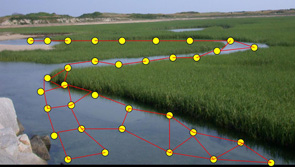
\includegraphics[scale = 2]{images/routing-river.jpg}
		\caption{Routing River}
		\label{fig:Routing River}
	\end{figure}

\section{Data Aggregation}

	The sensor nodes in the network often have limited resources, such as computation power, memory, storage, communication capacity and most significantly, battery power.
	The wireless data communications between nodes consume a large portion of the total energy consumption. 
	In-network data aggregation techniques allow the sensor nodes to aggregate the data before sending it to their parents.
	This technique reduces the wireless communication happening between the nodes and the overall energy consumption in the network. 	
	For example, in-network data aggregation of the SUM function can be performed as follows.
	All the intermediate sensor nodes in the network, receives the sensor readings from all of their children.
	They aggregate all those readings by applying the summation function to those readings.
	A network, which has the star topology, shown in Figure \ref{fig:star-network}, the root of the tree receives the following sensor readings $S_{1}(10),S_{2}(14),S_{3}(12),S_{4}(15),S_{5}(11),S_{6}(17)$.
	The root has its own reading of $S_{0}(15)$. 
	The root node aggregates these seven readings and creates an aggregated result as follows:
	\begin{equation}
		S = \sum_{i=0}^6 S_{i}
	\end{equation}
	Now, instead of sending all those sensor readings one at a time to its parent, it can send one aggregated sensor reading.
	In this example the aggregate function is summation, but it can be replaced with other statistical functions such as average, median, count etc., with little or no modification.
	\begin{figure}[h!]
		\centering
		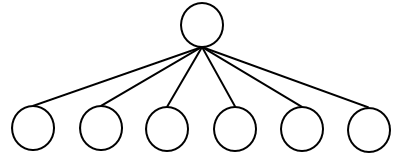
\includegraphics[scale = 1]{images/star-tree.png}
		\caption{Star Network}
		\label{fig:star-network}
	\end{figure}

	According to \cite{zareafifi2012secure}, \textbf{data aggregation} can be defined as follows.
	Consider a sensor network with $n$ sensors collecting data, the data will be propagated in some fashion to the base station.
	At the base station, the data is aggregated and processed into information. 
	This can be represented as
		$f(x_{1}, x_{2},...,x_{n})$
	where $x_{1}, x_{2},..., x_{n}$ represent the sensor readings.
	Here $f$ is some mapping $f: \mathcal{D}_{1} \times \mathcal{D}_{2} \times ... \mathcal{D}_{n}$ $\rightarrow$ $I$, where $\mathcal{D}_{i}$ represents sensor $i$'s domain and $I$ represents the set of all possible information. 
	Thus the goal is to compute the information as follows:
	\begin{equation}
		\label{eq:aggregation}
		y =\ f(x_{1}, x_{2},...,x_{n})
	\end{equation}

	It is shown that the energy savings achieved by in-network data aggregation are significant \cite{madden2002tag}.
	The in-network data aggregation approach requires the sensor nodes to do more computations.
	But studies have shown that wireless communication of data transmission requires more energy than local computation of the data. 
	In-network data aggregation is an efficient and a widely used approach for saving bandwidth by doing less wireless communications between sensor nodes and ultimately giving longer battery life to sensor nodes in the network.

	We define the following terms to help us define the goals of in-network data aggregation.
	\begin{definition}\label{def:payload}\cite{PayloadWiKi}
		\textbf{Payload} is the part of the transmitted data which is the fundamental purpose of the transmission, to the exclusion of information sent with it such as meta data solely to facilitate the delivery.
	\end{definition}
	\begin{definition}\label{def:information-rate}
		For a given node \textbf {Information rate} is the ratio of the number of sent payloads over the received payloads.
	\end{definition}
	The goal of the aggregation process is to achieve the lowest possible information-rate.
	In the following sections, we show that lowering information rate makes the intermediate sensor nodes (aggregator) more powerful.
	Also, it makes aggregated payload more fragile and vulnerable to various security attacks.

\section{Bandwidth Analysis}
	Congestion is a widely used parameter while doing bandwidth analysis of networking applications.
	% Picture
	% Definitions vs Equations errors 
	The congestion for any given node is defined as follows:
	\begin{equation}\label{def:congestion}
		Node\ congestion = Edge\ congestion \cdot Fanout
	\end{equation}
	Congestion is a useful factor while analyzing sensor network as it measures how quickly the sensor nodes will exhaust their batteries \cite{madden2003design}. 
	Some nodes in the sensor network have more congestion than the others, the highly congested nodes are the most important to the the network connectivity.
	For example, the nodes closer to the base station are essential for the network connectivity.
	The failure of the highly congested nodes may cause the sensor network to fail even though most of the nodes in the network are alive.
	Hence, it is desirable to have a lower congestion on the highly congested nodes even though it costs more congestion within the overall sensor network.
	To distribute the congestion uniformly across the network, we can construct an aggregation protocol where each node transmits a single payload as Definition \ref{def:payload} to its parent in the aggregation tree.
	In this approach, the fanout ($\delta$) depends on the given aggregation tree.
	For example, in the aggregation tree shown in Figure \ref{fig:star-network}, with $n$\ nodes, organized in the star tree topology, we see the congestion is $O(n)$.
	For the network organized in the palm tree topology, as shown in Figure \ref{fig:palm-tree-network}, the congestion is $\theta(1)$.
	\begin{figure}[h!]
		\centering
		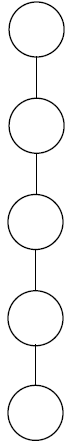
\includegraphics[scale = 1]{images/palm-tree.png}
		\caption{Palm Tree Network Topology}
		\label{fig:palm-tree-network}
	\end{figure}
	This approach can create some highly congested nodes in the aggregation tree which is undesirable.
	In most of the real world applications, we cannot control $\delta$ as the aggregation tree is random.
	Hence, it is desirable to have uniform distribution of congestion across the aggregation tree.

	Even though network topology can be random, in our observation, palm tree, star tree, binary tree are widely used network topologies to do the performance analysis.
	In the following chapters, we describe how to run our protocol for any random aggregation tree.
	In the end, we do bandwidth analysis of the protocol for star, palm and binary trees.

\section{Resilient And Non-Resilient Aggregate Functions}
	
	Wagner \cite{wagner2004resilient} uses statistical estimation theory to quantify the effects of direct data injection on various aggregates functions as follows:
	% Data aggregation definition should be in section 3.1

	% \begin{definition}
	% 	\cite{chan2006secure} Each sensor node $s_{i}$ has a data value $a_{i}$\ assuming that all the data values are non-negative bounded by real value $a_{i} \in [0,r]$, where $r$\ is the maximum allowed data value.
	% 	The objective of the \textbf{Aggregation Function} is to compute some function $f$ over all the data values, i.e., $f (a_{1}, \dotsc ,a_{n})$.
	% \end{definition}
	\begin{definition}
		\label{def:direct-data-injection}
		\cite{chan2006secure} A \textbf{Direct Data Injection} attack occurs when an adversary modifies the data readings reported by the nodes under its direct control, under the constraint that only legal readings in $[0, r]$ are reported.
	\end{definition}
	An \textbf{estimator} is an algorithm $ f :\ \R^n \rightarrow \rm I\!R$\ where $f(x_{1},\dotsc, x_{n})$\ is intended as an estimate of some real valued function of $\theta$.
	We assume that $\theta$ is real-valued and that we wish to estimate $\theta$ itself.
	Next, we define $\widehat{\Theta} := f(X_{1},\dotsc,X_{n})$, where $X_{1},\dotsc,X_{n}$\ are $n$ random variables. We can define the root-mean-square(r.m.s)  error (at $\theta$):
	\begin{equation}
		rms(f) := \rm I\!E[(\widehat{\Theta} - \theta)^2 | \theta]^{1/2}
	\end{equation}
	Note that r.m.s($f$) is a function of $\theta$; we compare functions pointwise. 
	Also, an unbiased estimator is one for which $E[\widehat{\Theta} | \theta] = \theta $ for all $\theta$.

	Wagner in \cite{wagner2004resilient} defines \textbf{resilient estimators and resilient aggregation } as follows.
	A \textbf{\textit{k}-node attack \textit{A}} is an algorithm that is allowed to change up to $k$ of the values $X_{1}, \dotsc, X_{n}$ before the estimator is applied.
	In particular, the attack $A$ is specified by a function $\tau_{A} : \R^n \rightarrow  \R^n $ with the property that the vectors $x$ and $\tau_{A}(x)$ never differ at more than $k$ positions.
	We can define the r.m.s error associated with $A$ as follows:
	\begin{equation}
		rms^*(f,A) := \rm I\!E[(\widehat{\Theta}^* - \theta)^2 | \theta]^{1/2} 		  
	\end{equation}
	where $\widehat{\Theta}^* := f(\tau_{A}(X_{1},\dotsc,X_{n}))$.
	To explain, $\widehat{\Theta}^*$\ is a random variable that represents the aggregate calculated at the base station in the presence of the $k$-node attack $A$, and $rms^*(f,A)$\ is a measure of inaccuracy of the aggregate after $A$'s intrusion.
	If $rms^*(f,A) \gg rms(f)$, then the attack has succeeded in noticeably affecting the operation of the sensor network.
	If $rms^*(f,A) \approx rms(f)$, the attack had little or no effect.
	We define
	\begin{equation}
		rms^*(f,k) := max\{rms^*(f,A): A\ is\ a\ k-node\ attack\}
	\end{equation}
	so that $rms^*(f,k)$\ denotes the r.m.s. error of the most powerful
	$k$-node attack possible. 
	Note that $rms^* (f, 0) = rms(f)$.
	We think of an aggregation function $f$ as an instance of the resilient aggregation paradigm if $rms^* (f, k)$ grows slowly as a function of $k$.
	\begin{definition}
		\cite{wagner2004resilient} An aggregation function $f$ is \textbf{$(k, \alpha)$-resilient} (with respect to a parameterized distribution $p(X_{i} | \theta))$ if $rms^*(f, k) \le \alpha \cdot rms(f)$ for the estimator $f$.
		\label{def:resilient}
	\end{definition}
	The intuition is that the $(k, \alpha)$-resilient functions, for small values of $\alpha$, are the ones that can be computed meaningfully and securely in the presence of up to $k$ compromised or malicious nodes.
	According to this quantitative study measuring the effects of direct data injection on various aggregates, concludes that the \textbf{aggregates (truncated SUM and AVERAGE ) can be resilient} under such attacks.
	Wagner's work is summarized in the following Table.
	\begin{table}[!htb]	
		\begin{center}
		\caption{Summary of Wagner's work}
			\begin{tabular}{ |l| l| }
				\hline
			    Aggregate(f) & Security Level \\
			    \hline
			    minimum & insecure \\
			    maximum & insecure \\
			    sum & insecure \\
				average & insecure \\
				count & acceptable \\
				$[l,u]$-truncated average & problematic \\
				5\% -trimmed average & better \\
				median & much better \\
			    \hline
			\end{tabular}
		\end{center}
		\label{table:wagner}
	\end{table}

\section{Security Issues}
	\label{sec:security-issues}
	
	The aggregation schemes can be compared with compression schemes.
	``Lossless data compression'' \cite{alberto2000communication} produces a compressed file from which the original data can be recovered exactly.
	Facsimile uses lossless data compression.
	However, lossless data compression schemes are limited in the compression rates they can achieve.
	``Lossy data compression'' \cite{alberto2000communication} schemes produces a compressed file from which only an approximation to the original information can be recovered. Much higher compression ratios are possible.
	The aggregation scheme will be a \textit{lossy data compression} because once the base station receives the final aggregated value it can not create the original sensor readings of the sensor nodes.
	Hence, it is very important that the base station has very high confidence in the received final aggregated value. 
	For example, in Equation \ref{eq:aggregation} Sensor \rom{2}'s reading is changed from $x_{2}$ (the ``true reading'') to $x'_{2}$ by an intermediate aggregator, then an aggregate node computes $y' =\ f(x_{1},x'_{2},...,x_{n})$.
	It is very likely that $y' \neq y$ where $y$ is the true information if the true reading was counted.
	The base station takes an action based on the received information $y'$.
	How dangerous would it be to act using $y'$?
	Thus, if one ``knows there is some likelihood of false data'' how do we protect the information generated?


	As we know, in-network data aggregation technique saves bandwidth by transmitting less payloads between sensor nodes thus increasing the lifetime of the network.
	Designing one such protocol for the sensor networks poses a numerous challenges due to resource limitations and inherent characteristics discussed in the previous chapter.	
	Moreover, this technique empowers intermediate aggregate sensor nodes in the network by allowing them to control certain portion of the network.
	A malicious intermediate sensor node who does aggregation over all of its descendants payloads, needs to tamper with only one aggregated payload instead of tampering with all the payloads received from its descendants. 
	Thus, a malicious intermediate sensor node needs to do less work to skew the final aggregated payload.
	An adversary controlling few sensor nodes in the network can cause the network to return unpredictable payloads, making an entire sensor network unreliable.
	Intermediate sensor nodes adversarial power is proportional to their number of descendants.

	While applying the data-aggregation techniques the integrity of the sensor readings becomes more valuable.
	As one or few faulty sensor readings can deviate the final aggregated result.
	For example,
	% Fail to safe operation	
	% Suppose $n$ seismic sensors are collecting seismic readings \cite{zareafifi2012secure}.
	% The sensor data is then processed to compute $y = f(x_{1},..., x_{n})$ where $y = (y_{1}, y_{2})$, here $y_{1}$ represents the time prediction of an earthquake and $y_{2}$ represents the duration of the earthquake. Suppose $y^* = (y^*_{1}, y^*_{2})$, where $y^*$ is the approximate (or faulty) information.
	% Then to measure the quality we need to compute $|y - y^*|$, but observe that many of the common metrics fail to capture the essence of the prediction (it is more important to determine date than duration).
	% Thus a metric that measure the quality of the approximation must make sense. 
	% It is possible that the best measure of the essence of the computation does not possess all the	properties of a metric.
	National Snow and Ice Data Center on June $3, 2008$ \cite{nsidc} reported that Arctic sea ice extent had declined through the month of May as summer approaches. 
	Daily ice extents in May continued to be below the long-term average and approached the low levels seen at the same time last year.
	The spring ice cover was thin, one sign of thin and fairly weak ice was the formation of several polynyas in the ice pack.
	The Defense Meteorological Satellite Program (DMSP) F13 \cite{dmsp-f13} satellite, which had been central to their Arctic sea ice analysis for the past several years, is nearing the end of its mission.
	As the standard data practice, they have transitioned to a newer sensor, in that case the DMSP F15 \cite{dmsp-f15}. 
	The DMSP F15 had the same type of sensor as the DMSP F13. 
	NSIDC had done preliminary inter calibration to assure consistency with the historical record. 
	They said that due to the inter calibration errors the final reported ice extent values might differ on average $\pm 30,000$ square kilometers or $11,600$ square miles per preliminary number reported.
	The faulty sensor readings can be caused due to malfunctioning sensors, the active attacks on true sensor readings or incorrect interpretations of the data, which can cause catastrophic situations.
	Hence, it is necessary to take countermeasures while using data-aggregation techniques.

	Despite the fact that in-network aggregation makes an intermediate sensor nodes more powerful and aggregated value more vulnerable to various security attacks, some aggregation approaches requires strong network topology assumptions or honest behaviors from the sensor nodes.
	For example, in-network aggregation schemes in \cite{yao2002cougar, madden2003design} assumes that all the sensor nodes in the network are honest. 
	Secure Information Aggregation (SIA) of \cite{przydatek2003sia} enables secure information aggregation such that the user accepts the data with high probability if the aggregated result is within a desired bound, but that the user detects cheating with high probability and rejects the result if it is outside of the bound.
	The SIA provides probabilistic security for the network topology with a single-aggregate model.

	An approach to detection and diagnosis of multiple failures in a dynamic system is proposed in \cite{zhang1998detection}. 
	It is based on the Interacting Multiple-Model (IMM) estimation algorithm, which is one of the most cost-effective adaptive estimation techniques for systems involving structural as well as parametric changes. 
	The proposed approach provides an integrated framework for fault detection, diagnosis, and state estimation. 
	It is able to detect and isolate multiple faults substantially more quickly and more reliably than many existing approaches. 
	Its superiority is illustrated in two aircraft examples for single and double faults of both sensors and actuators, in the forms of total, partial, and simultaneous failures. 

	Secure hierarchical in-network aggregation (SHIA) in sensor networks \cite{chan2006secure} presents the first and provably secure sensor network data aggregation protocol for general networks and multiple adversaries. 
	We discuss the details of the protocol in the next chapter. 
	SHIA limits the adversary's ability to tamper with the aggregation result with the tightest bound possible.
	But it does not help detecting an adversary in the network.
	We build our work on the foundation of SHIA, which allows to track down the adversary and remove it from the network.